\subsubsection{u.1 Registrazione di un nuovo utente}

Dopo aver determinato il volume dei dati ed aver associato a ciascuna operazione principale richiesta la frequenza di esecuzione procediamo ad esaminare gli schemi di navigazione per le principali operazioni richieste.
\begin{longtblr}
[
  caption = {Registrazione di un nuovo utente},
]{
  colspec = {|X[3]X[1]X[2]X[4]|},
  rowhead = 1,
  hlines,
  row{even} = {lightgray},
  row{1} = {LightCoral},
} 
Concetto & Costrutto & Accessi & Tipo\\
Users & E & 1 & Scrittura \\
% \multicolumn{4}{|c|}{Totale: 1S \textrightarrow 500/giorno}
&  & Totale: 1S \textrightarrow 300/giorno & 

\end{longtblr}


\subsubsection{u2. Login di un utente}
\begin{longtblr}
[
  caption = {Login di un utente},
]{
  colspec = {|X[3]X[1]X[2]X[4]|},
  rowhead = 1,
  hlines,
  row{even} = {lightgray},
  row{1} = {LightCoral},
} 
Concetto & Costrutto & Accessi & Tipo\\
Users & E & 1 & L\\ 
& & Totale: 1L \textrightarrow 1500/giorno &
\end{longtblr}

\subsubsection{u3. Modificare i dati del proprio account}
\begin{longtblr}
  [
    caption = {Modificare i dati del proprio account},
  ]{
    colspec = {|X[3]X[1]X[2]X[4]|},
    rowhead = 1,
    hlines,
    row{even} = {lightgray},
    row{1} = {LightCoral},
  } 
  Concetto & Costrutto & Accessi & Tipo\\
  Users & E & 1 & L\\ 
  & & Totale: 1S \textrightarrow 300/giorno &
  \end{longtblr}


%%%%%% ADMIN %%%%%%%
\subsubsection{a1. Consultare la lista degli enti}
Per ogni ente recupero l'utente che lo ha creato e la media delle recensioni.\\
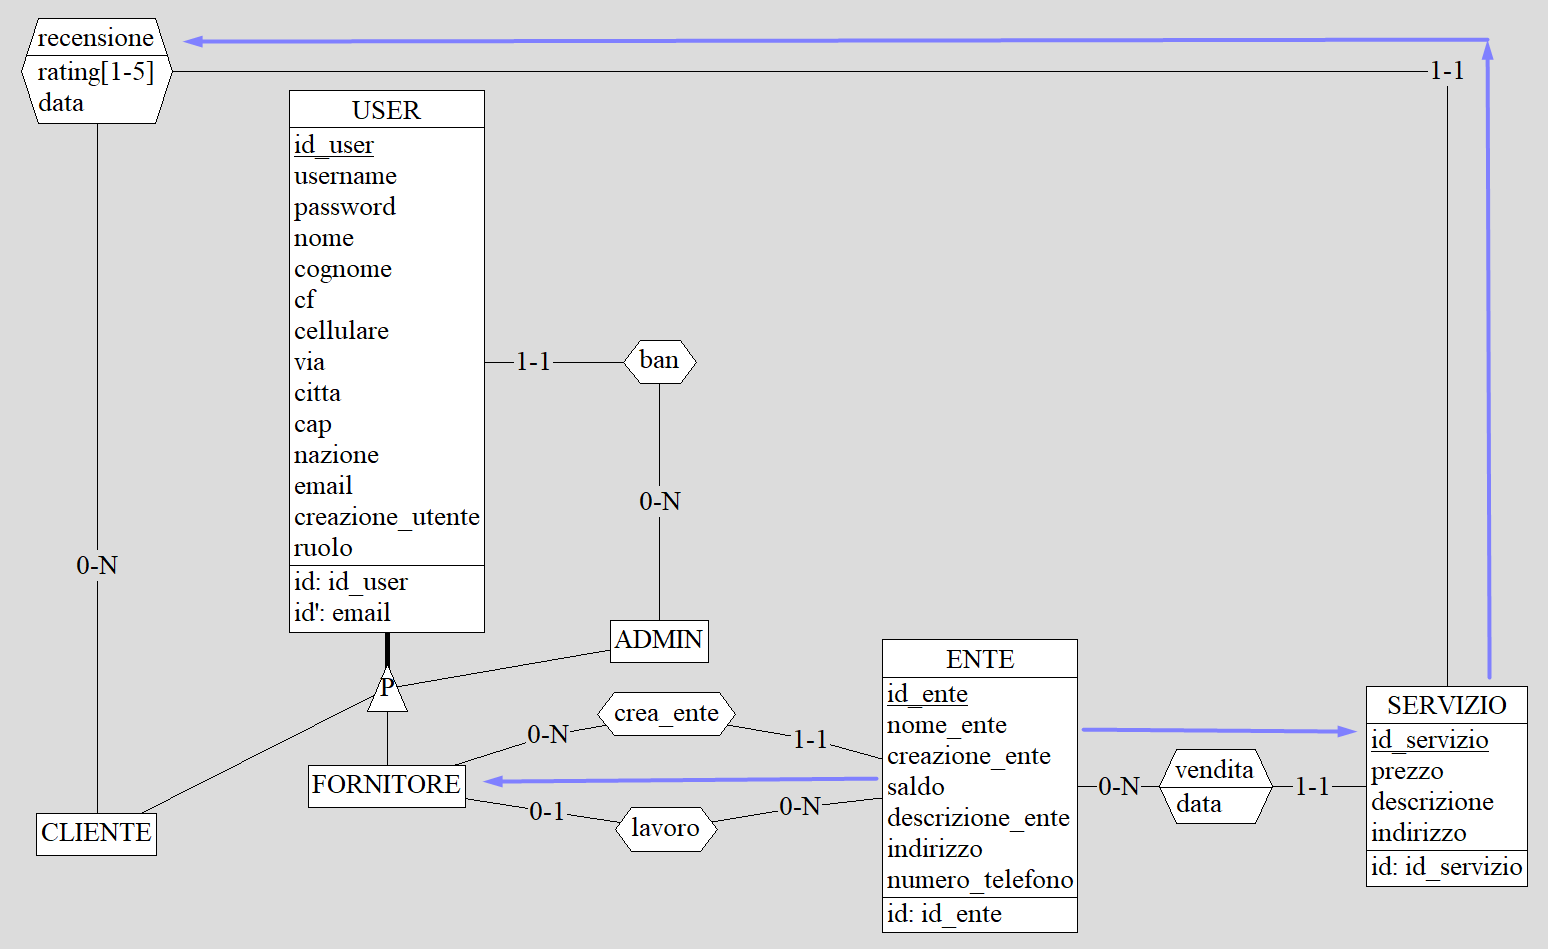
\includegraphics[width=0.95\columnwidth]{a1getUser.png}
\begin{longtblr}
  [
    caption = {Consultare la lista degli enti},
  ]{
    colspec = {|X[3]X[1]X[2]X[4]|},
    rowhead = 1,
    hlines,
    row{even} = {lightgray},
    row{1} = {LightCoral},
  } 
  Concetto & Costrutto & Accessi & Tipo\\
  Users & E & 1 & L\\ 
  & & Totale: 4L \textrightarrow 50/giorno &
  \end{longtblr}


  \subsubsection{a2. Bannare gli altri utenti}
  \begin{longtblr}
    [
      caption = {Bannare gli altri utenti},
    ]{
      colspec = {|X[3]X[1]X[2]X[4]|},
      rowhead = 1,
      hlines,
      row{even} = {lightgray},
      row{1} = {LightCoral},
    } 
    Concetto & Costrutto & Accessi & Tipo\\
    Users & E & 1 & L\\ 
    & & Totale: 1S \textrightarrow 5/giorno &
    \end{longtblr}


%%% TODO 
\begin{longtblr}
[
caption = {a3. Reset delle recensioni},
]{
colspec = {|X[3]X[1]X[2]X[4]|},
rowhead = 1,
hlines,
row{even} = {lightgray},
row{1} = {LightCoral},
} 
Concetto & Costrutto & Accessi & Tipo\\
Users & E & 1 & L\\ 
& & Totale: 1S \textrightarrow 5/giorno &
\end{longtblr}


Verranno eseguite le query necessarie per ottenere le seguenti statistiche:\\
\begin{itemize}
  \item numero check-in
  \item numero check-in falliti
  \item numero CityCard attive
  \item numero eventi attivi
  \item numero servizi attivi
\end{itemize}
\begin{longtblr}
[
caption = {a4. Consultare statistiche},
]{
colspec = {|X[3]X[1]X[2]X[4]|},
rowhead = 1,
hlines,
row{even} = {lightgray},
row{1} = {LightCoral},
} 
Concetto & Costrutto & Accessi & Tipo\\
Users & E & 1 & L\\ 
& & Totale: 5L \textrightarrow 5/giorno &
\end{longtblr}



\begin{longtblr}
[
caption = {f1. Creare enti},
]{
colspec = {|X[3]X[1]X[2]X[4]|},
rowhead = 1,
hlines,
row{even} = {lightgray},
row{1} = {LightCoral},
} 
Concetto & Costrutto & Accessi & Tipo\\
Users & E & 1 & L\\ 
& & Totale: 1S \textrightarrow 2/giorno &
\end{longtblr}

\begin{longtblr}
[
caption = {f2. Associarsi a un ente},
]{
colspec = {|X[3]X[1]X[2]X[4]|},
rowhead = 1,
hlines,
row{even} = {lightgray},
row{1} = {LightCoral},
} 
Concetto & Costrutto & Accessi & Tipo\\
Users & E & 1 & L\\ 
& & Totale: 1S \textrightarrow 3/giorno &
\end{longtblr}


\begin{longtblr}
[
caption = {f3. Creare servizi},
]{
colspec = {|X[3]X[1]X[2]X[4]|},
rowhead = 1,
hlines,
row{even} = {lightgray},
row{1} = {LightCoral},
} 
Concetto & Costrutto & Accessi & Tipo\\
Users & E & 1 & L\\ 
& & Totale: 1L + 1S \textrightarrow \num{10}/giorno &
\end{longtblr}

\begin{longtblr}
[
caption = {f4. Creare eventi occasionali},
]{
colspec = {|X[3]X[1]X[2]X[4]|},
rowhead = 1,
hlines,
row{even} = {lightgray},
row{1} = {LightCoral},
} 
Concetto & Costrutto & Accessi & Tipo\\
Users & E & 1 & L\\ 
& & Totale: 1L + 1S \textrightarrow \num{4}/giorno &
\end{longtblr}



Per creare un evento periodico si dovrà ottenere l'id dell'ente al quale è associato il fornitore, poi andare a creare un record per l'evento e un altro record per il periodo. \\
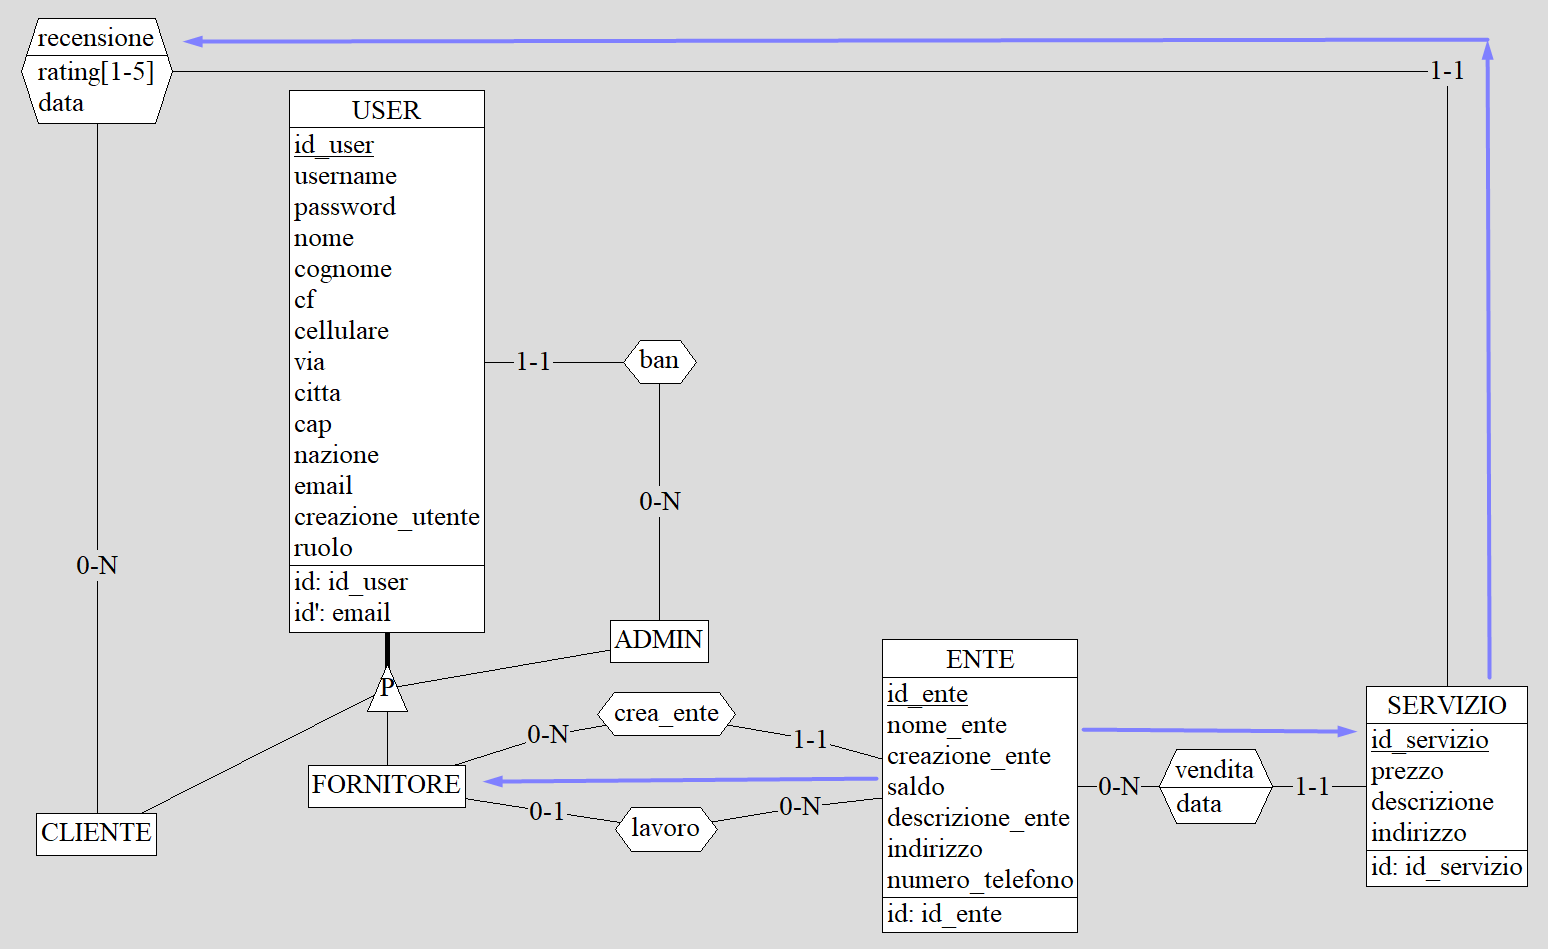
\includegraphics[width=0.95\columnwidth]{a1getUser.png}
\begin{longtblr}
[
caption = {f5. Creare eventi periodici},
]{
colspec = {|X[3]X[1]X[2]X[4]|},
rowhead = 1,
hlines,
row{even} = {lightgray},
row{1} = {LightCoral},
} 
Concetto & Costrutto & Accessi & Tipo\\
Users & E & 1 & L\\ 
& & Totale: 1L + 2S \textrightarrow \num{1}/giorno &
\end{longtblr}



Oltre alla query per ottenere il'id dell'ente del fornitore verranno eseguite quelle necessarie per ottenere le seguenti statistiche:\\
\begin{itemize}
  \item saldo dell'ente associato al fornitore
  \item numero eventi attivi
  \item numero servizi attivi
\end{itemize}
\begin{longtblr}
[
caption = {f6. Consultare statistiche riguardo il proprio ente},
]{
colspec = {|X[3]X[1]X[2]X[4]|},
rowhead = 1,
hlines,
row{even} = {lightgray},
row{1} = {LightCoral},
} 
Concetto & Costrutto & Accessi & Tipo\\
Users & E & 1 & L\\ 
& & Totale: 4L  \textrightarrow \num{800}/giorno &
\end{longtblr}

\begin{longtblr}
[
caption = {c1. Richiedere una CityCard},
]{
colspec = {|X[3]X[1]X[2]X[4]|},
rowhead = 1,
hlines,
row{even} = {lightgray},
row{1} = {LightCoral},
} 
Concetto & Costrutto & Accessi & Tipo \\
Users & E & 1 & L\\ 
& & Totale: 1S  \textrightarrow \num{2000}/giorno &
\end{longtblr}

Prima di sottoscrivere un abbonamento vengono cercate una CityCard valida e una carta di credito predefinita. \\
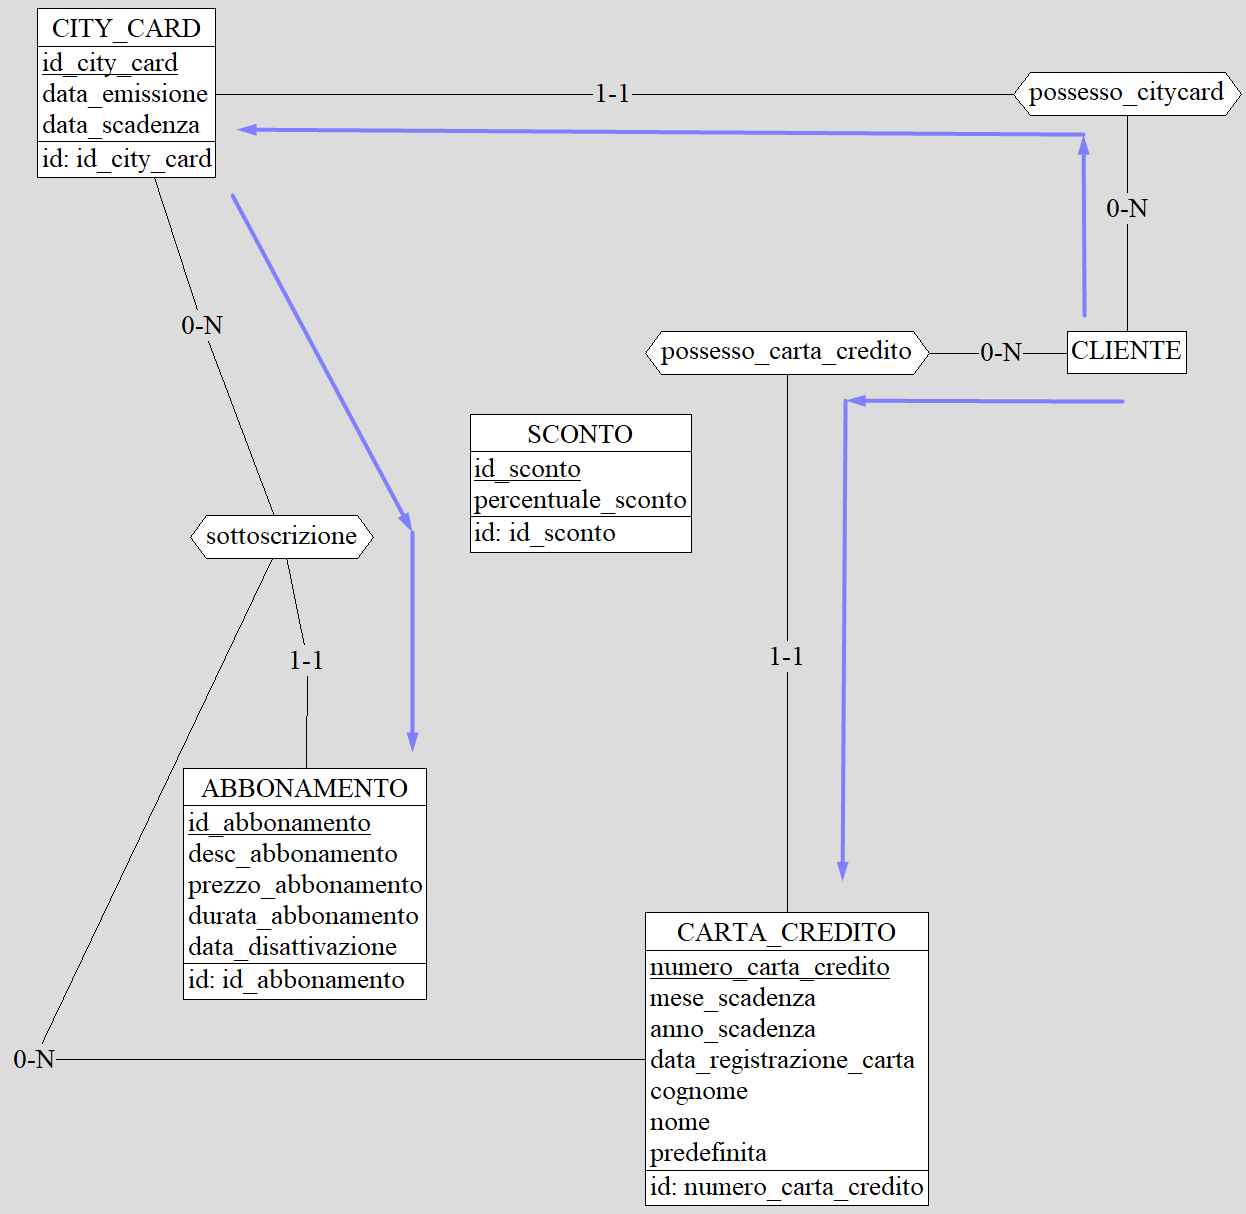
\includegraphics[width=0.95\columnwidth]{c2sottoscrizioneAbbonamento.png}
\begin{longtblr}
[
caption = {c2. Sottoscrivere un abbonamento},
]{
colspec = {|X[3]X[1]X[2]X[4]|},
rowhead = 1,
hlines,
row{even} = {lightgray},
row{1} = {LightCoral},
} 
Concetto & Costrutto & Accessi & Tipo \\
Users & E & 1 & L\\ 
& & Totale: 2L+1S  \textrightarrow \num{2000}/giorno &
\end{longtblr}

\begin{longtblr}
[
caption = {c3. Aggiungere una carta di credito},
]{
colspec = {|X[3]X[1]X[2]X[4]|},
rowhead = 1,
hlines,
row{even} = {lightgray},
row{1} = {LightCoral},
} 
Concetto & Costrutto & Accessi & Tipo \\
Users & E & 1 & L\\ 
& & Totale: 1S  \textrightarrow \num{2000}/giorno &
\end{longtblr}

\begin{longtblr}
[
caption = {c3. Aggiungere una carta di credito},
]{
colspec = {|X[3]X[1]X[2]X[4]|},
rowhead = 1,
hlines,
row{even} = {lightgray},
row{1} = {LightCoral},
} 
Concetto & Costrutto & Accessi & Tipo \\
Users & E & 1 & L\\ 
& & Totale: 1S  \textrightarrow \num{2000}/giorno &
\end{longtblr}

\begin{longtblr}
[
caption = {c4. Aggiungere una carta di credito},
]{
colspec = {|X[3]X[1]X[2]X[4]|},
rowhead = 1,
hlines,
row{even} = {lightgray},
row{1} = {LightCoral},
} 
Concetto & Costrutto & Accessi & Tipo \\
Users & E & 1 & L\\ 
& & Totale: 1S  \textrightarrow \num{2000}/giorno &
\end{longtblr}


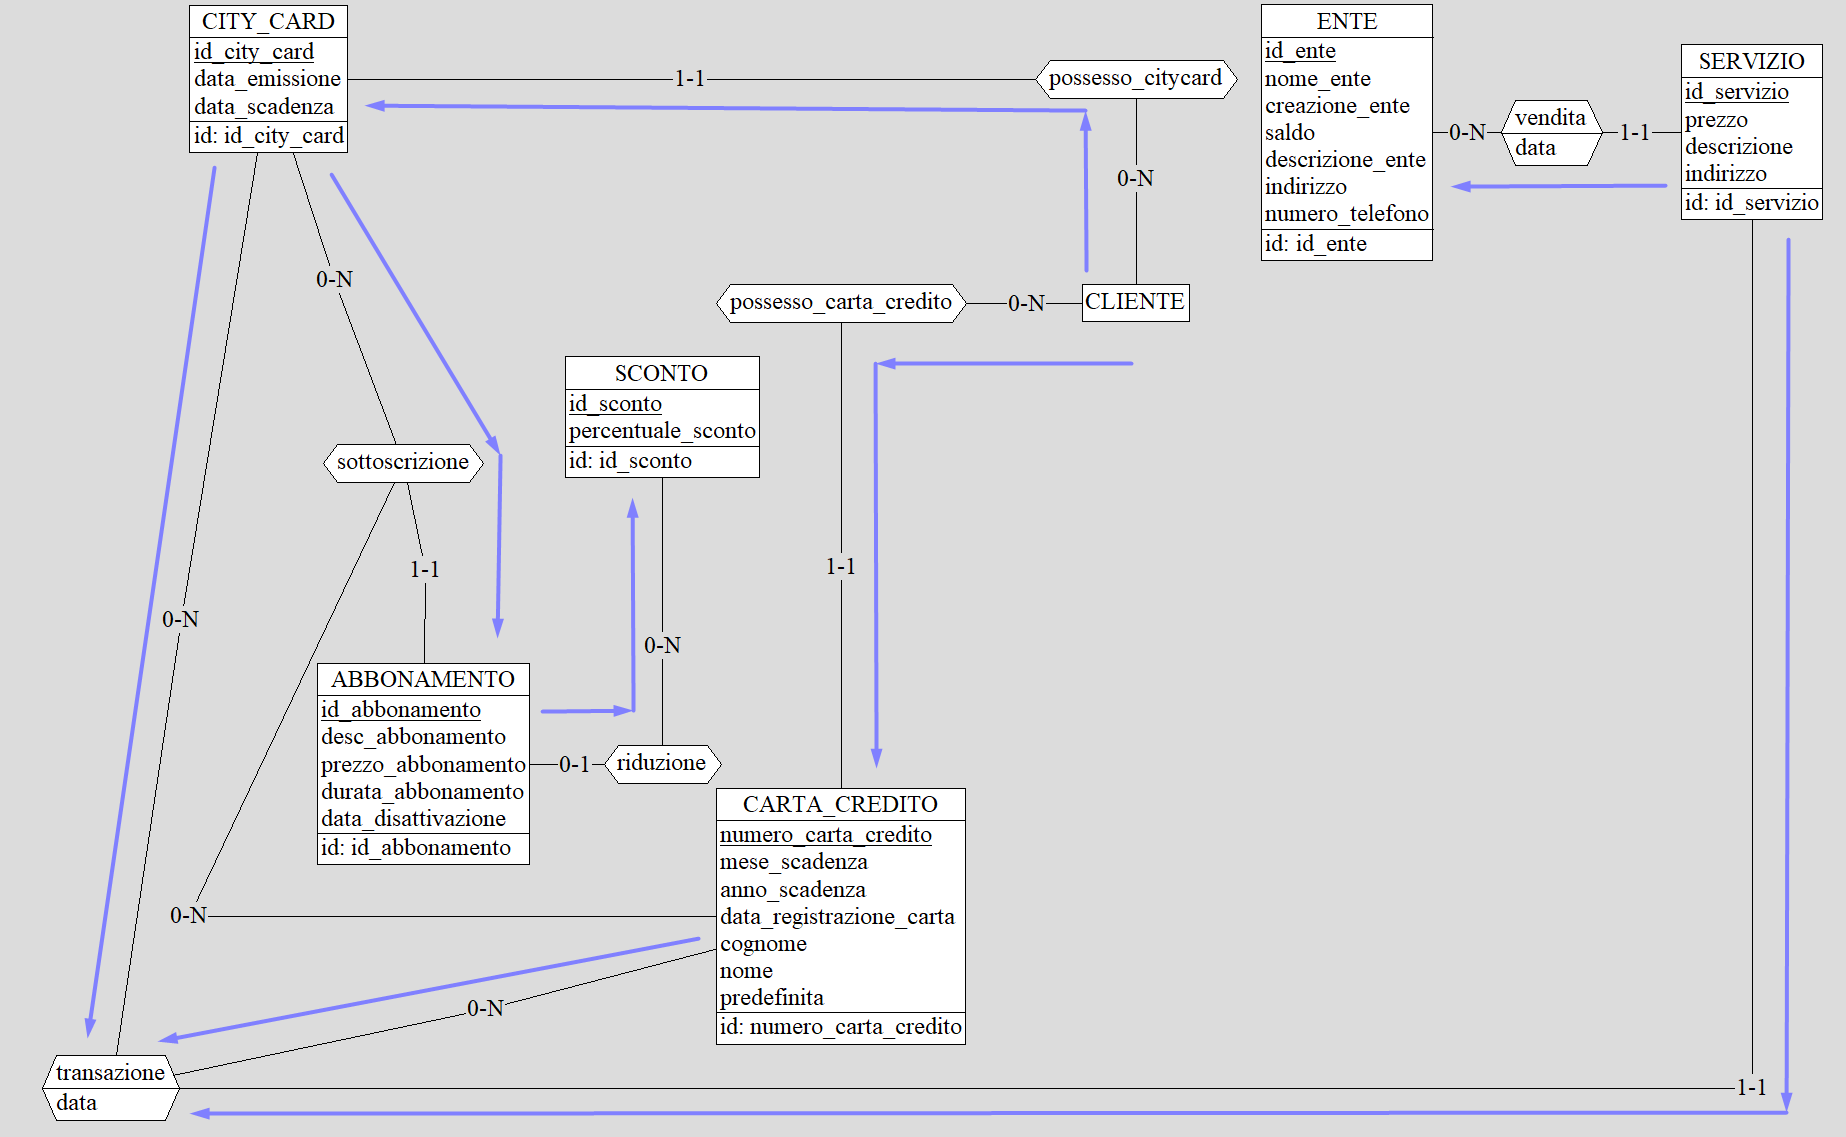
\includegraphics[width=0.95\columnwidth]{c5acquistaServizio.png}
\begin{longtblr}
[
caption = {c5. Acquistare un servizio},
]{
colspec = {|X[3]X[1]X[2]X[4]|},
rowhead = 1,
hlines,
row{even} = {lightgray},
row{1} = {LightCoral},
} 
Concetto & Costrutto & Accessi & Tipo \\
Enti & E & 1 & L\\ 
Servizi & E & 1 & L\\ 
Carta di credito & E & 1 & L\\ 
CityCard & E & 1 & L\\ 
Sconti & E & 1 & L\\ 
Abbonamenti & E & 1 & L\\ 
Sottoscrizione & E & 1 & L\\ 
Servizi & E & 1 & L\\ 
Transazione & E & 1 & R\\ 
& & Totale: 8L + 1S  \textrightarrow \num{3000}/giorno &
\end{longtblr}


\begin{longtblr}
[
caption = {c6. Prenotare un evento},
]{
colspec = {|X[3]X[1]X[2]X[4]|},
rowhead = 1,
hlines,
row{even} = {lightgray},
row{1} = {LightCoral},
} 
Concetto & Costrutto & Accessi & Tipo \\
Eventi & E & 1 & L\\ 
& & Totale: 1S \textrightarrow \num{500}/giorno &
\end{longtblr}


Per poter effettuare un check-in devo confermare che la CityCard del cliente sia valida.
\begin{longtblr}
[
caption = {c7. Effettuare un check-in},
]{
colspec = {|X[3]X[1]X[2]X[4]|},
rowhead = 1,
hlines,
row{even} = {lightgray},
row{1} = {LightCoral},
} 
Concetto & Costrutto & Accessi & Tipo \\
CityCard & E & 1 & L\\ 
Checks & E & 1 & L\\   % CAMBIARE
& & Totale: 1L + 1S \textrightarrow \num{5000}/giorno &
\end{longtblr}

\begin{longtblr}
[
caption = {c8. Consultare la lista degli acquisti fatti},
]{
colspec = {|X[3]X[1]X[2]X[4]|},
rowhead = 1,
hlines,
row{even} = {lightgray},
row{1} = {LightCoral},
} 
Concetto & Costrutto & Accessi & Tipo \\
servizi acquistati & E & 1 & L\\ 
CityCard & E & 1 & L\\ 
User & E & 1 & L\\ 
Servizi & E & 1 & L\\ 
& & Totale: 4L\textrightarrow \num{3000}/giorno &
\end{longtblr}


%% TODO  calcolare ridondanze
\begin{longtblr}
[
caption = {c9. Lasciare una recensione riguardo un servizio acquistato},
]{
colspec = {|X[3]X[1]X[2]X[4]|},
rowhead = 1,
hlines,
row{even} = {lightgray},
row{1} = {LightCoral},
} 
Concetto & Costrutto & Accessi & Tipo \\
servizi acquistati & E & 1 & L\\ 
CityCard & E & 1 & L\\ 

& & Totale: 4L\textrightarrow \num{1500}/giorno &
\end{longtblr}

% TODO Capire se può tornare utile
\begin{longtblr}
  [
    caption = {Cliente recensisce servizio},
  ]{
    colspec = {|X[3]X[1]X[2]X[4]|},
    rowhead = 1,
    hlines,
    row{even} = {lightgray},
    row{1} = {LightCoral},
  } 
  Concetto & Costrutto & Accessi & Tipo\\
  
  Cliente & E &  & L\\ 
  Recensisce & R &  & S \\
  Servizio & E & & S \\
  & & Totale: \textrightarrow  & 
  \end{longtblr}



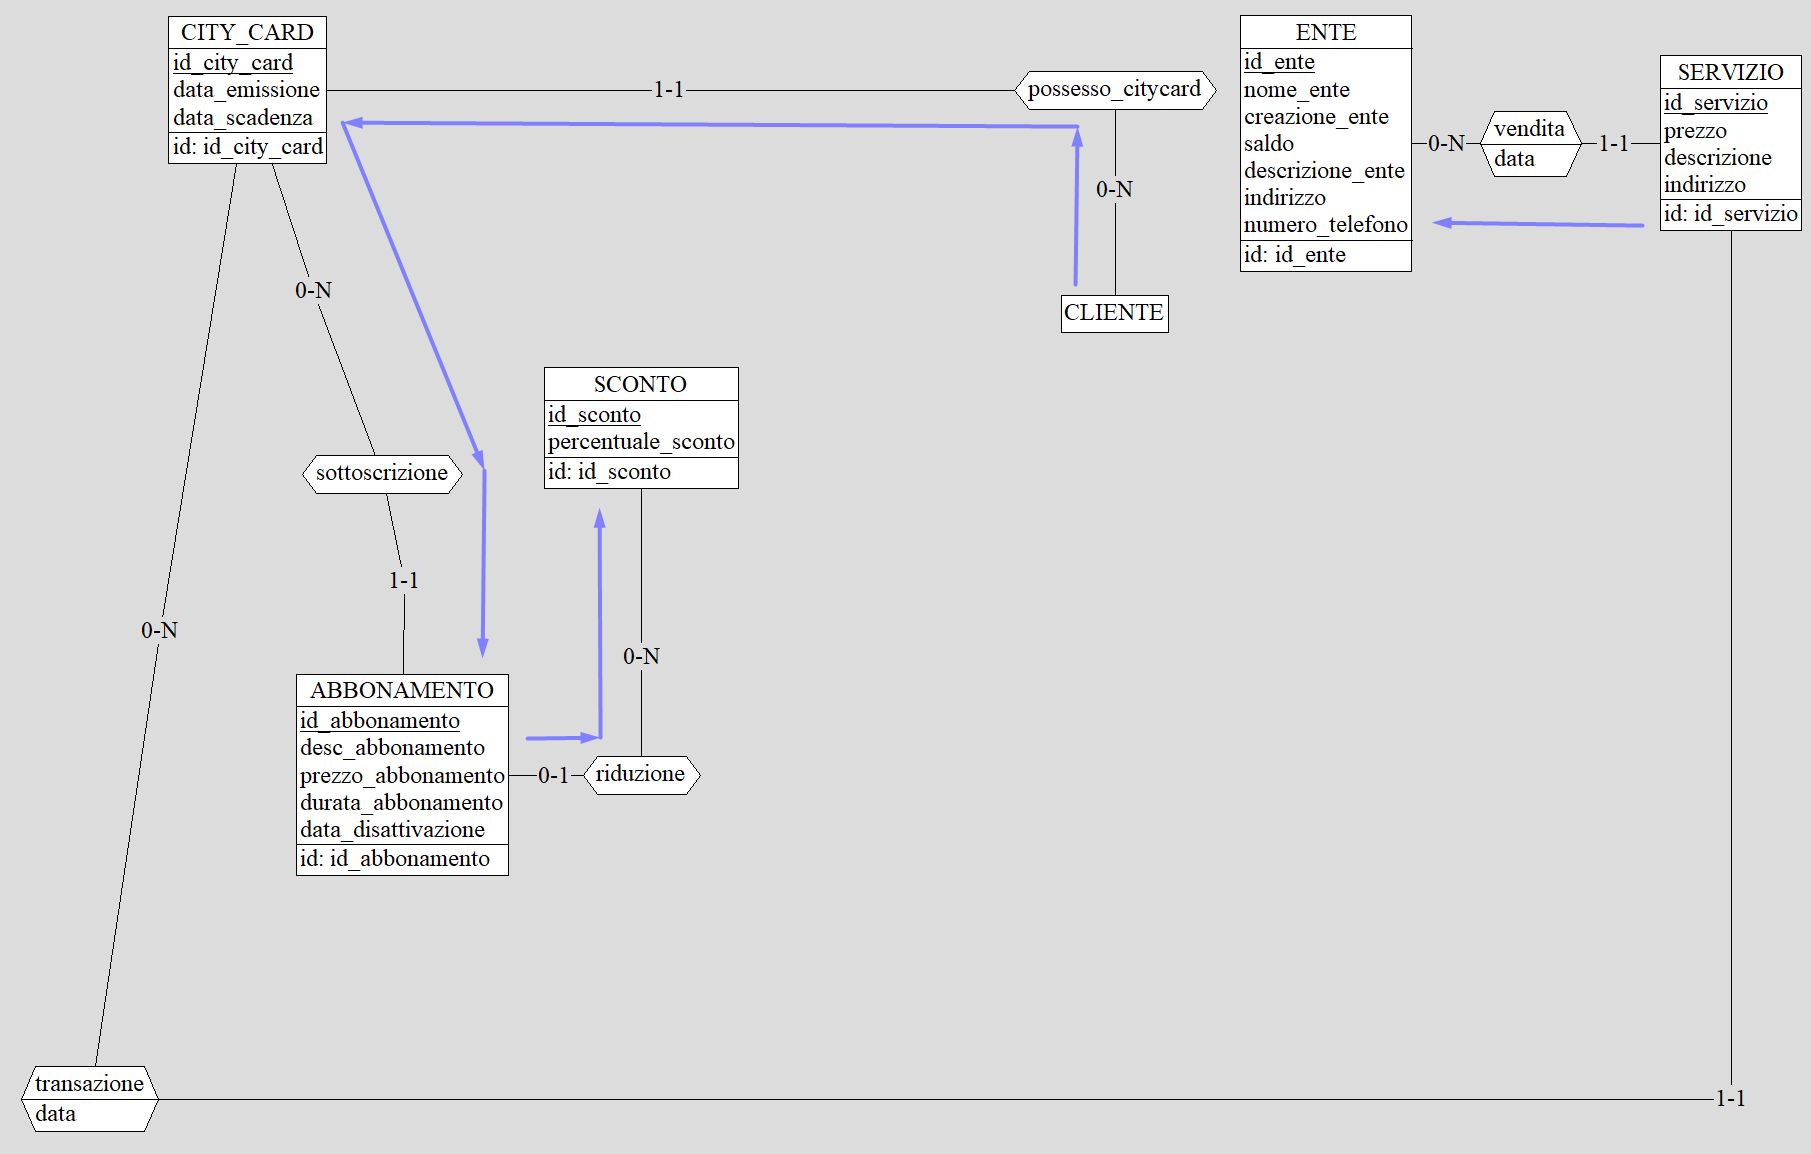
\includegraphics[width=0.95\columnwidth]{c10getServizi.png}
Nella tabella dei servizi disponibili si dovrà mettere anche l'ente fornitore, il prezzo scontato in base all'abbonamento sottoscritto dal cliente.
\begin{longtblr}
[
caption = {c10. Visualizzare lista servizi},
]{
colspec = {|X[3]X[1]X[2]X[4]|},
rowhead = 1,
hlines,
row{even} = {lightgray},
row{1} = {LightCoral},
} 
Concetto & Costrutto & Accessi & Tipo \\
CityCard & E & 1 & L\\ 
sconti & E & 1 & L\\ 
listino abbonamenti & E & 1 & L\\ 
sottoscrizione abbonamenti & E & 1 & L\\ 
servizi & E & 1 & L\\ 
enti & E & 1 & L\\ 

& & Totale: 6L\textrightarrow \num{7500}/giorno &
\end{longtblr}


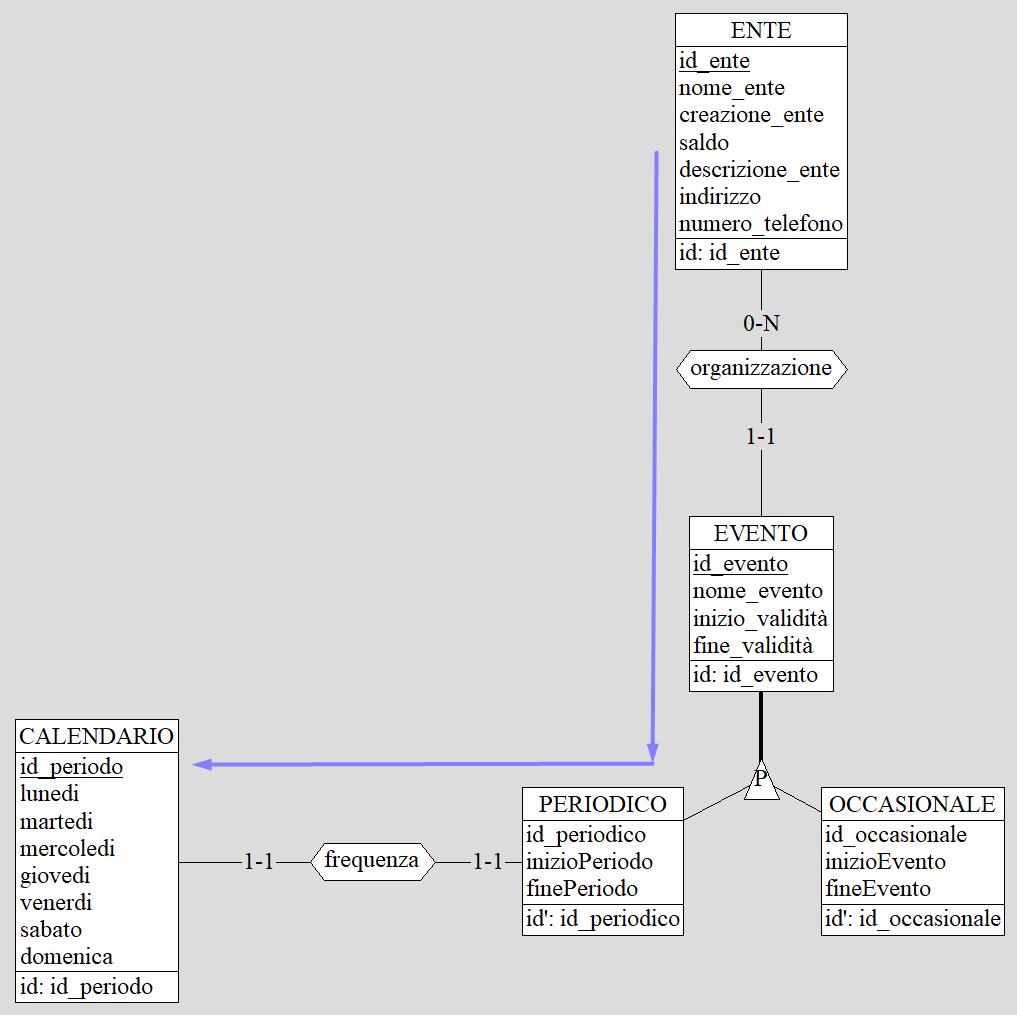
\includegraphics[width=0.95\columnwidth]{c11getEventi.png}
Nella tabella dei servizi disponibili si dovrà mettere anche l'ente fornitore, il prezzo scontato in base all'abbonamento sottoscritto dal cliente.
\begin{longtblr}
[
caption = {c11. Visualizzare lista eventi},
]{
colspec = {|X[3]X[1]X[2]X[4]|},
rowhead = 1,
hlines,
row{even} = {lightgray},
row{1} = {LightCoral},
} 
Concetto & Costrutto & Accessi & Tipo \\
eventi & E & 1 & L\\ 
periodi & E & 1 & L\\ 
enti & E & 1 & L\\ 

& & Totale: 3L\textrightarrow \num{1500}/giorno &
\end{longtblr}


% TODO Decidere se lasciare come extra
\begin{longtblr}
[
  caption = {Visualizzazione lista carta di credito},
]{
  colspec = {|X[3]X[1]X[2]X[4]|},
  rowhead = 1,
  hlines,
  row{even} = {lightgray},
  row{1} = {LightCoral},
} 
Concetto & Costrutto & Accessi & Tipo\\

Cliente & E & 1 & L\\ 
Possiede & R & 2 & L \\
Carta di credito & E & 2 & L \\
& & Totale: 5L \textrightarrow 10000/settimana & \\
\end{longtblr}

